\section{Proposed data architecture}

\begin{figure}
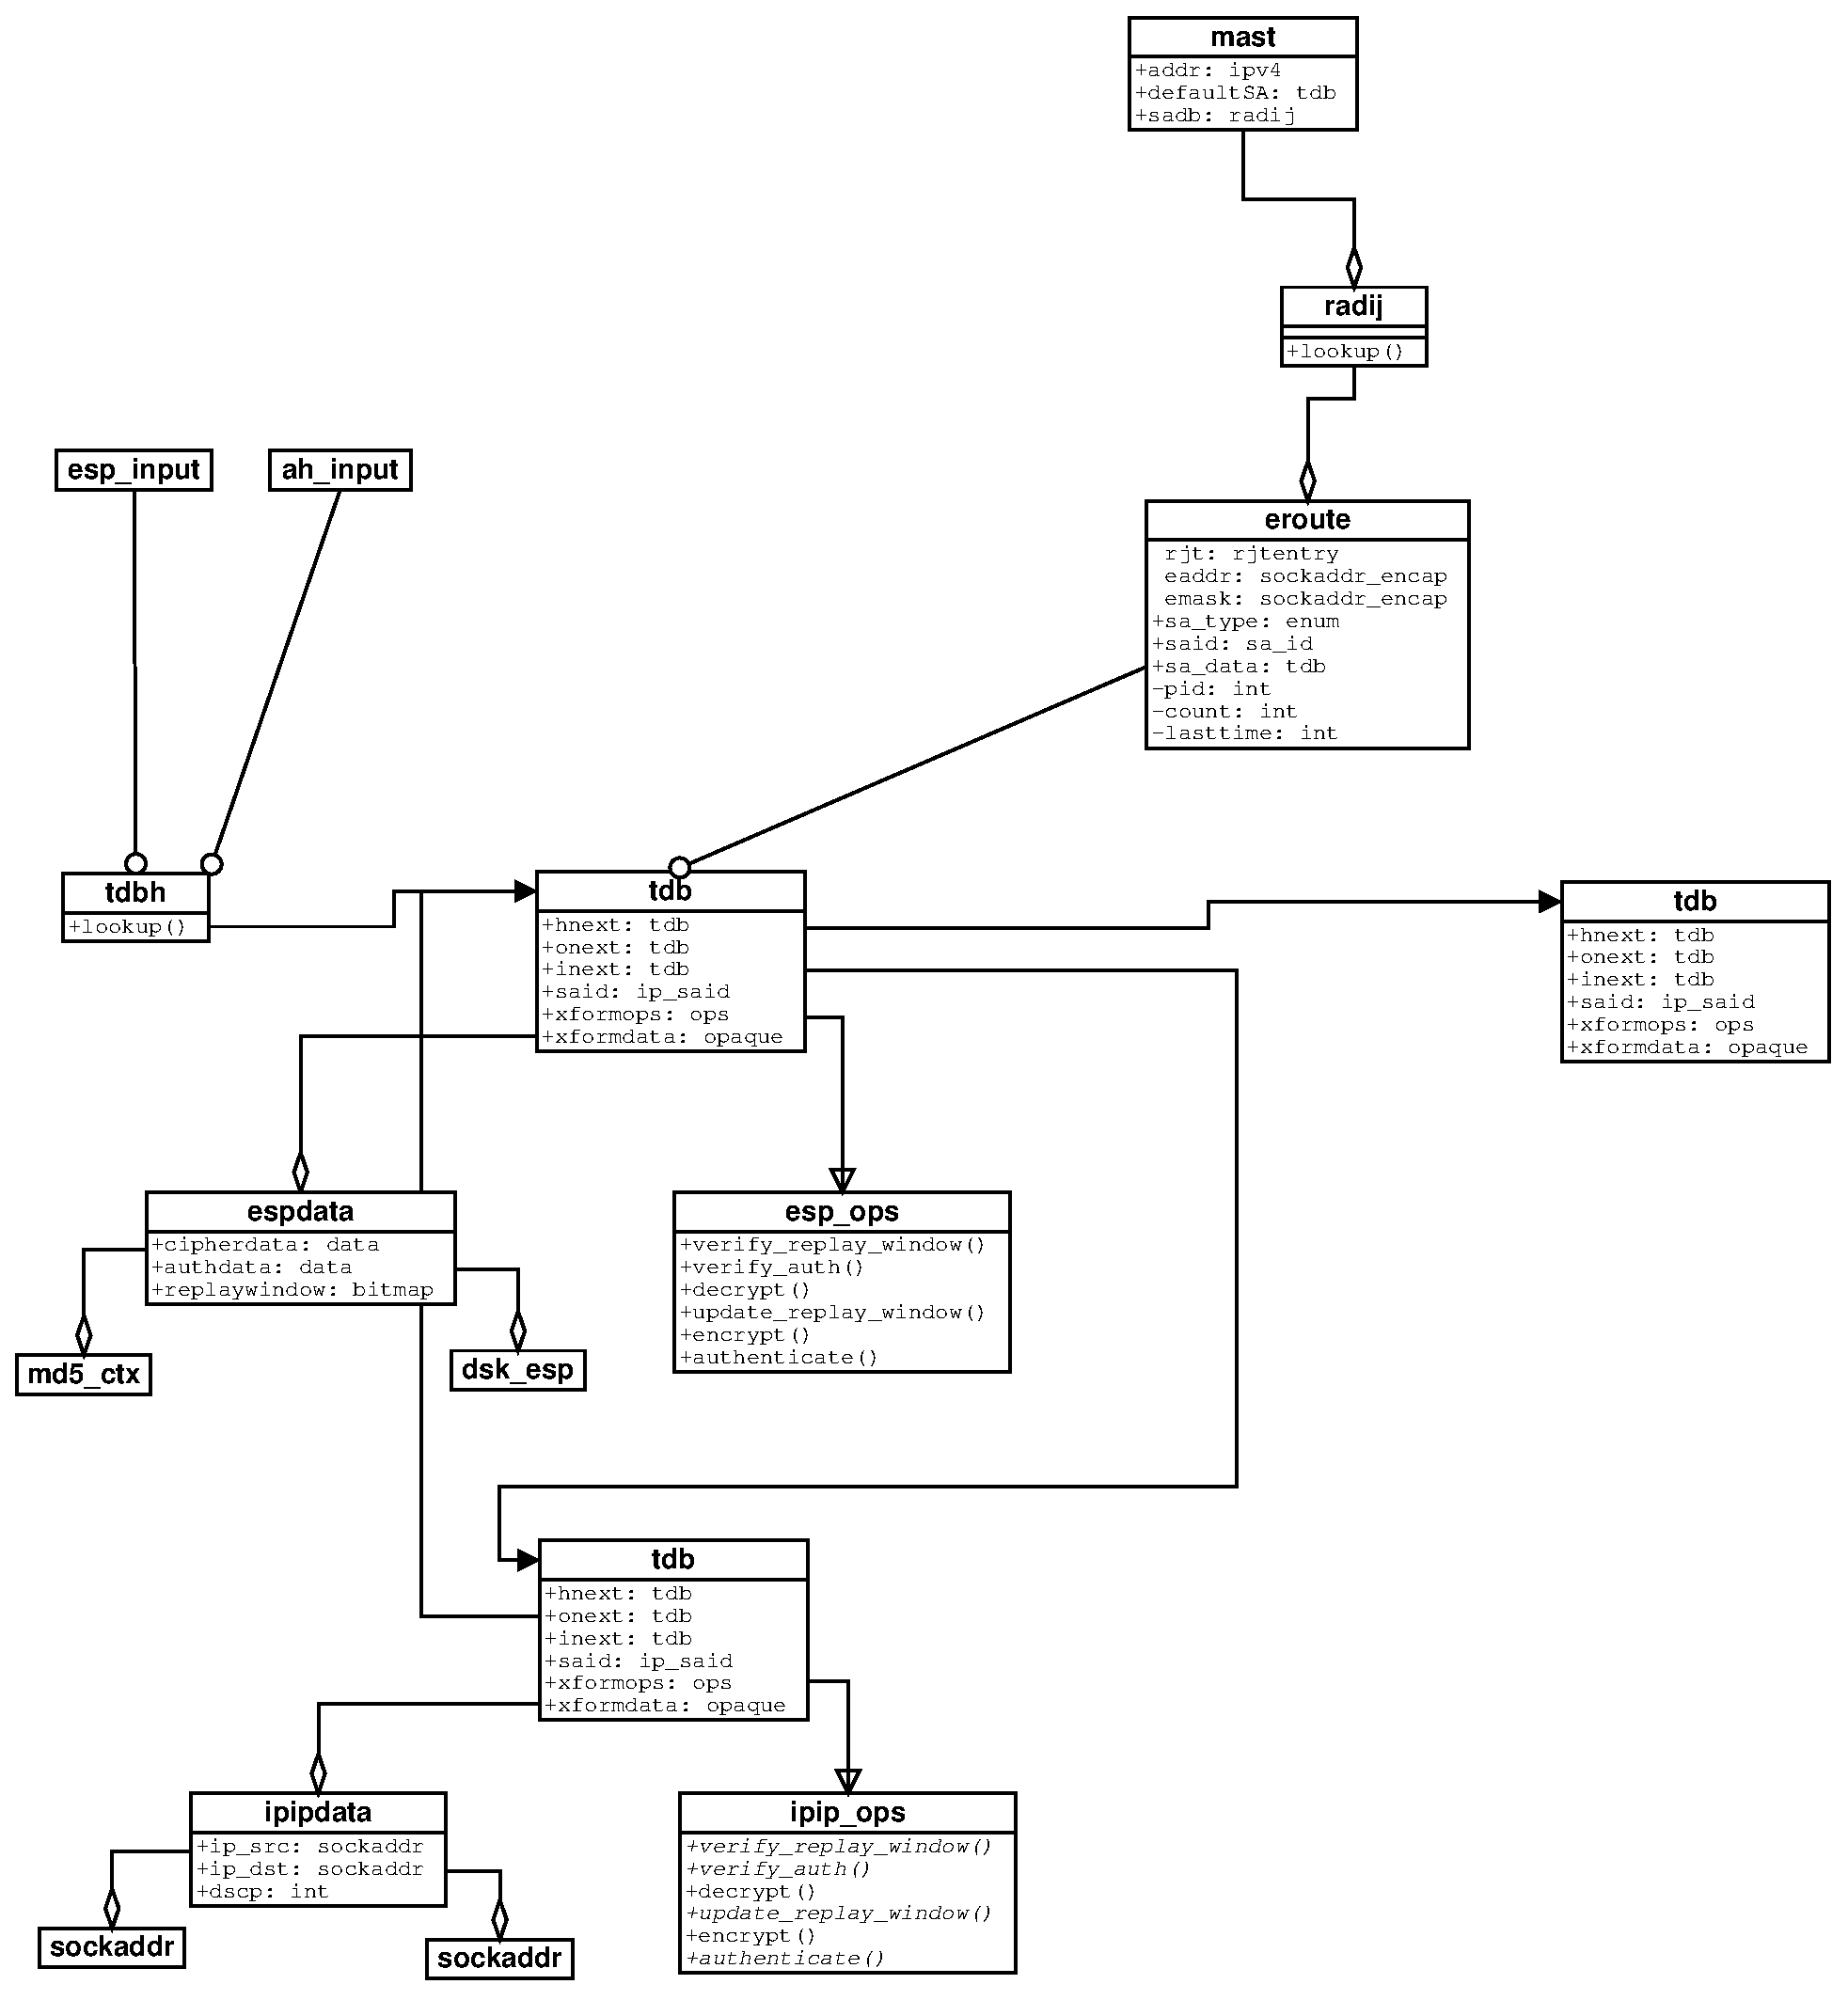
\includegraphics[height=6in,width=6in]{diagrams/klips2_tdb.eps} 
\label{KLIPS2 data structures}
\end{figure}

\subsection{klips2 mast}

The MAST device provide a mooring point for routing protocols and firewall
policies. The MAST device represents one or more IPsec tunnels. 

Packets routed to a MAST device will get encrypted with a default SA.
A different SA may be specified using NetFilter (aka ipchains, aka iptables)
rules. 

Packets that are received via one of the SAs associated with this device
will be marked as having been received on a MAST device. 

The link status of a MAST device reflects the keying status of all underlying 
SAs. If at least one SA is keyed, then the MAST device will be up. If no SA
that is associated has valid keys, or if no SAs that are associated with the
device, then the device will be marked down.

This is provided in part to satisfy requirement 21 (see \ref{req021})
and requirement 5 (see \ref{req005}).

\subsection{klips2 radij}

The radij tree provides a lookup on eroute entities.  

While the eroute database provides the IPsec security policy database (SPD),
the radij tree is the index into it by selectors.

It is a BSD radix.c derived table. It has been modified to permit masking of
bits of the index to occur in arbitrary places, thus permitting both source
and destination addresses to be masked.

The radij tree will be replaced or augmented to support additional selectors.
These include UDP/TCP port numbers, SPI numbers (for multiple layers of
gateways), ICMP types and codes, and possibly also IPSO labels.

As opportunistic encryption creates large numbers of fully specified
source/destination pairs, it will be investigated if an auxiliary table could
provide a more efficient storage of these tables. Specifically, it is
possible that connection tracking can more efficiently provide this required
index. 

\subsection{klips2 eroute}

The eroute is the object that represents an entry in the IPsec SPD.

This structure will be extended with additional selectors to support
requirement 11 (see \ref{req011}).

\subsection{klips2 ipsec\_sa\_buckethead}

This is the root of the transform database hash table. 

This structure is the renamed {\tt tdbh}.

\subsection{klips2 esp\_input}

The current {\tt ipsec\_rcv} will be cloned to create an ESP receive
function.

\subsection{klips2 ah\_input}

The current {\tt ipsec\_rcv} will be cloned to create an AH receive function.

\subsection{klips2 ipsec\_sa}

This is the renamed {\tt tdb} structure.

\subsection{klips2 espdata}

This is a per-SA structure that records all the information needed by the
algorithm database functions to perform their functions.

\subsection{klips2 esp\_ops}

This is the set of pointers to functions needed to perform the ESP steps.

\subsection{klips2 md5\_ctx}

This is a subpiece of the espdata structure that stores MD5 keys.

\subsection{klips2 ipipdata}

This structure provides information needed by the IPIP transform.

\subsection{klips2 ipip\_ops}

This is the set of pointers to functions needed to perform IPIP steps.
